\chapter{Materials and Methods}\label{chap:methods}

\section{Galaxy Platform}\label{sec:galaxy}
Galaxy is a web-based scientific platform that has become a major player in many fields of life sciences and bioinformatics. Founded in 2007 it has provided an emerging amount of resources and tools to empower scientists and researchers to work with biomedical datasets. The platform is free to use and collaborative, making it one of the biggest of its kind. Resources on Galaxy cover genomics, metagenomics, transcriptomics, proteomics, drug discovery and non-biology fields like natural language processing and social sciences.

Galaxy's primary objective is to make analyses more accessible, reproducible, and easier to communicate among researchers. The platform's distinctive and success is attributed to four core elements: a very active community, a public server for analyses, an open-source software ecosystem, and the Galaxy ToolShed. The community adheres to the FAIR practices (Findable, Accessible, Interoperable and Reusable)~\cite{10.1093/nar/gkac247}.

The Galaxy community is thriving, with over 124,000 users who also contribute to subcommunities. The public server for analyses provides access to public datasets and workflows. The open-source software ecosystem ensures automated setup and deployment of all tools and services, making it simple for beginners and professionals to use. The Galaxy ToolShed is a server dedicated to hosting, sharing, and installing tools used on the platform. A Galaxy tool is the abstraction layer that makes external software usable from within Galaxy with a frontend, i.e. lets users use the program with all its parameters and inputs from within Galaxy. \\ 
Galaxy workflows are a key feature that allow the user to stack tools in a chain and to configure them so that the workflow user only has to upload his or her data for the input fields. The automation of tools in a chain is used for modular, longer analyses that are executed repeatedly. \\
Workflows that are available on and accepted by the Intergalactic Workflow Commission (IWC; \url{https://github.com/galaxyproject/iwc}) are conform with the community's best practise standards and tested on the latest Galaxy release. Dockstore and WorkflowHub automatically publish the IWC workflows and guarantee the availability in a Docker-based environment on Dockstore~\cite{o2017dockstore} and on the workflow collaboratory WorkflowHub~\cite{goble2021implementing}.

Important contributions of Galaxy, as stated by the Galaxy Community (2022), include Vertebrate Genome Project assembly workflows and collaborations on SARS-CoV-2 research. Another toolkit leveraged in Galaxy is Galaxy-ML, a set of tool that provides a suite for analyses based on machine learning. With growing publicity, more topics are covered by and moved to Galaxy. It has contributed to over 5,700 scientific publications and has many tutorials available for researchers to use. Training material and ready-to-use workflows facilitate professionals and beginners in the field to use Galaxy for their research purposes.

The platform is continuously enhanced, and it still attracts around 2,000 new users every month, indicating the quality and significance of the project. The team and infrastructure of Galaxy initially come from the Nekrutenko lab in the Center for Comparative Genomics and Bioinformatics at Penn State, the Taylor lab at Johns Hopkins University, and the Goecks Lab at Oregon Health \& Science University. All of these organisations have contributed significantly to the success of Galaxy. There are 138 public servers available worldwide as of 2023, while the most prominent general-purpose server instances are hosted by teams at University of Freiburg, Germany (for \href{https://usegalaxy.eu/}{UseGalaxy.eu}), Texas Advanced Computing Center (for \href{https://usegalaxy.org/}{UseGalaxy.org}) and Genomics Virtual Laboratory, formerly at the University of Queensland (for \href{https://usegalaxy.org.au/}{UseGalaxy.org.au}). These main public servers are synchronized in their tools and set of reference tools~\cite{10.1093/nar/gkac247}.

\section{Requirements}

SARS-CoV-2 Pipeline as Baseline. \\
annotated variants are of interest \\
description of basic steps

\begin{figure}[ht!]
	\centering
	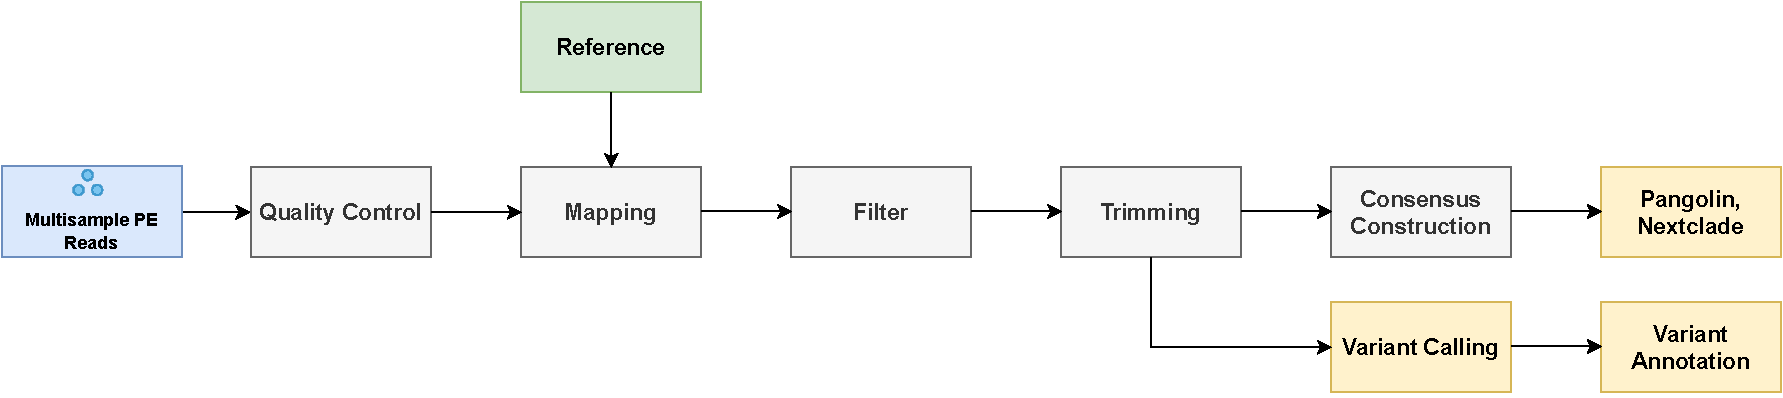
\includegraphics[width=0.97\textwidth]{media/3-pipelines-SARS-CoV-2.pdf}
	\caption{Simplified SARS-CoV-2 ARTIC PE reads iVar-based workflow.}
	\label{fig:3-pipelines-sars}
\end{figure}

tested workflow, includes 'minimal' steps:
\begin{enumerate}
	\item Quality control
	\item Mapping
	\item Filtering
	\item Trimming
	\item Consensus Sequence Construction
\end{enumerate}

Plus Variant Calling and genome annotation; \\
Plus phylogenetic ranking ''to assign a SARS-CoV-2 genome sequence the most likely lineage based on a chosen nomenclature system'' (Pangolin)

\begin{figure}[H]
	\centering
	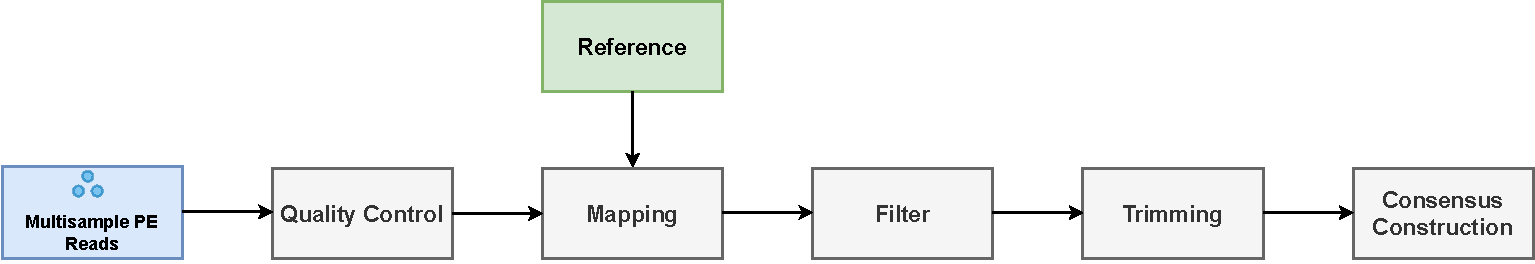
\includegraphics[width=0.97\textwidth]{media/3-pipelines-minimal.pdf}
	\caption{Simplified minimal ARTIC PE reads iVar-based workflow.}
	\label{fig:3-pipelines-minimal}
\end{figure}


which problems should the pipeline solve?

what is "ampliconic" sequence analysis, ARTIC Illumina-sequenced data

\subsubsection{Requirements for Poxvirus Workflow}
- repetitions in the start and end regions → need to split reads into 2 pools and mask references \\
- after splitting, merging alignments back

\subsubsection{Requirements for AIV Workflow}
- reference for each of the 8 segments has to be chosen \\
- align reference of each segment with consensus sequence and add to phylogenetic analysis \\
- snipit for visualisation of SNPs \\
- trimming would dismiss too many of the already short reads \\
- have a reference database ready for VAPOR (multifasta) with read name pattern \\
- dismiss B/C/D strains and H17, H18 subtypes (occur in bats only)
\\ a tool to get closest reference

For a detailed genetic analysis of the AIV genome, several consecutive steps are required after taking a sample from an infected host and sequencing it. NGS data need to be preprocessed in order to remove reads that are too short, have low base quality or include NGS platform-specific adapters that are ligated to the read ends and need to be trimmed.

why mapping is good and not assembly:
The diversity of HA and NA segments' sequences is significant enough to make it challenging to map sequenced reads to a single Influenza A reference sequence chosen by the user using a naive approach. Although this approach may be effective for the other six segments, the mapping software would frequently be unable to locate sufficient plausible matches for sequenced reads of HA and NA origin to continue with the analysis.

\subsubsection{Requirements for FMDV Workflow}

\section{Workflow Development}
''Reference-based genomic Surveillance'' (INSaFLU)

\subsection{Poxvirus Illumina Amplicon Workflow}
47 distinct steps

Tiling amplicon approach for CaPV genome. Makes up 23 primer pairs for an amplicon size of 7.5 kb each instead of smaller sizes usually used in tiling amplicon protocols. (ref2.2.2)

Workflow is composed of seven crucial steps:
- preparing reference sequence for mapping (masking halves)
- quality control
- mapping
- Filtering
- merging
- trimming
- consensus sequence construction

CaPV genomes have the central coding region bounded by identical inverted terminal repeats,
containing 156 putative genes. the repeat of the ITRs would make any mapping in these regions ambiguous.
need to part the reads in two pools and do mapping in two parts: N-mask the reference (start and end by start/end position primers)

\begin{figure}[H]
	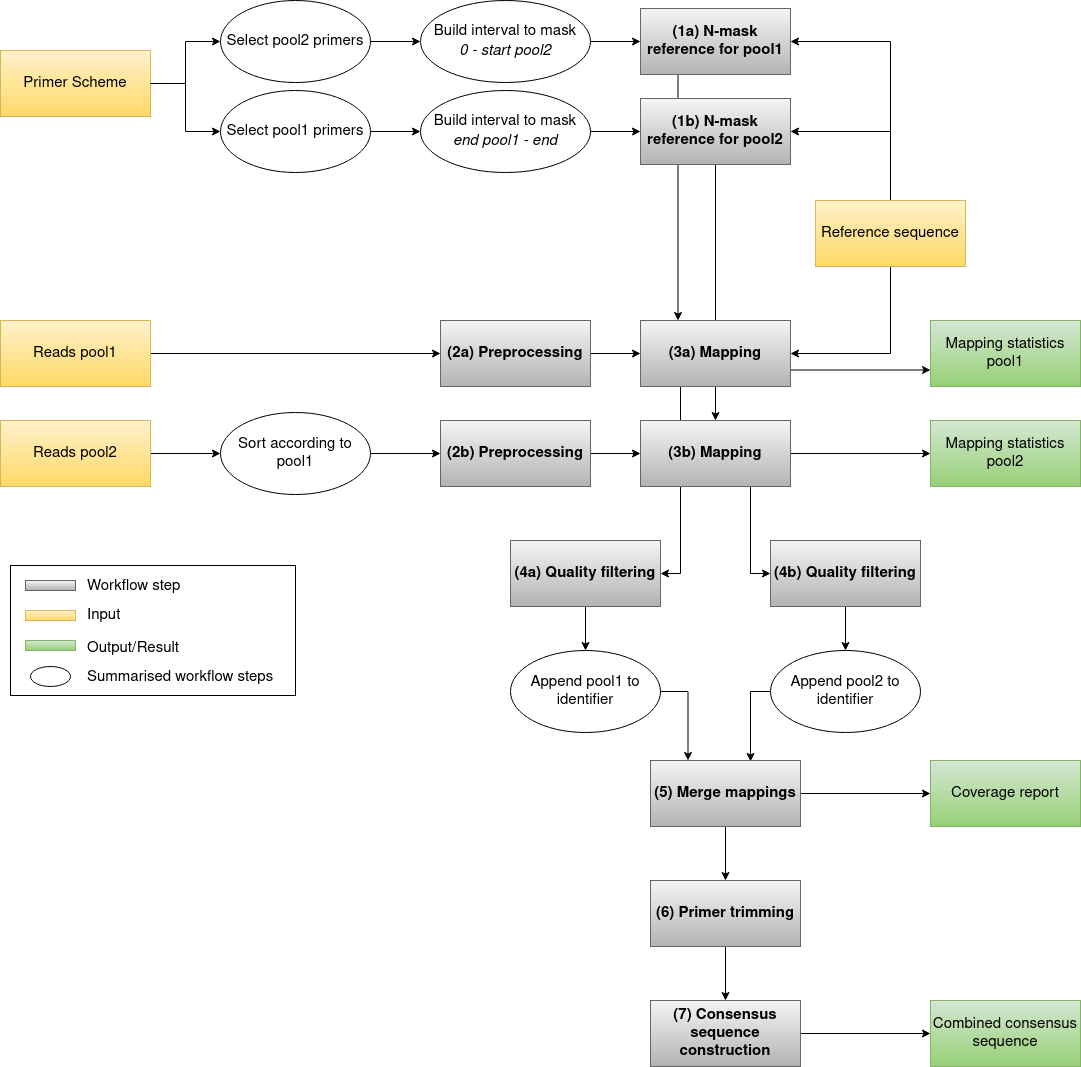
\includegraphics[width=1\textwidth]{media/pox.png}
	\caption{Simplified Poxvirus PE reads iVar-based workflow.}
	\label{fig:3-pox-wf}
\end{figure}

% \begin{figure}[H]
% 	\centering
% 	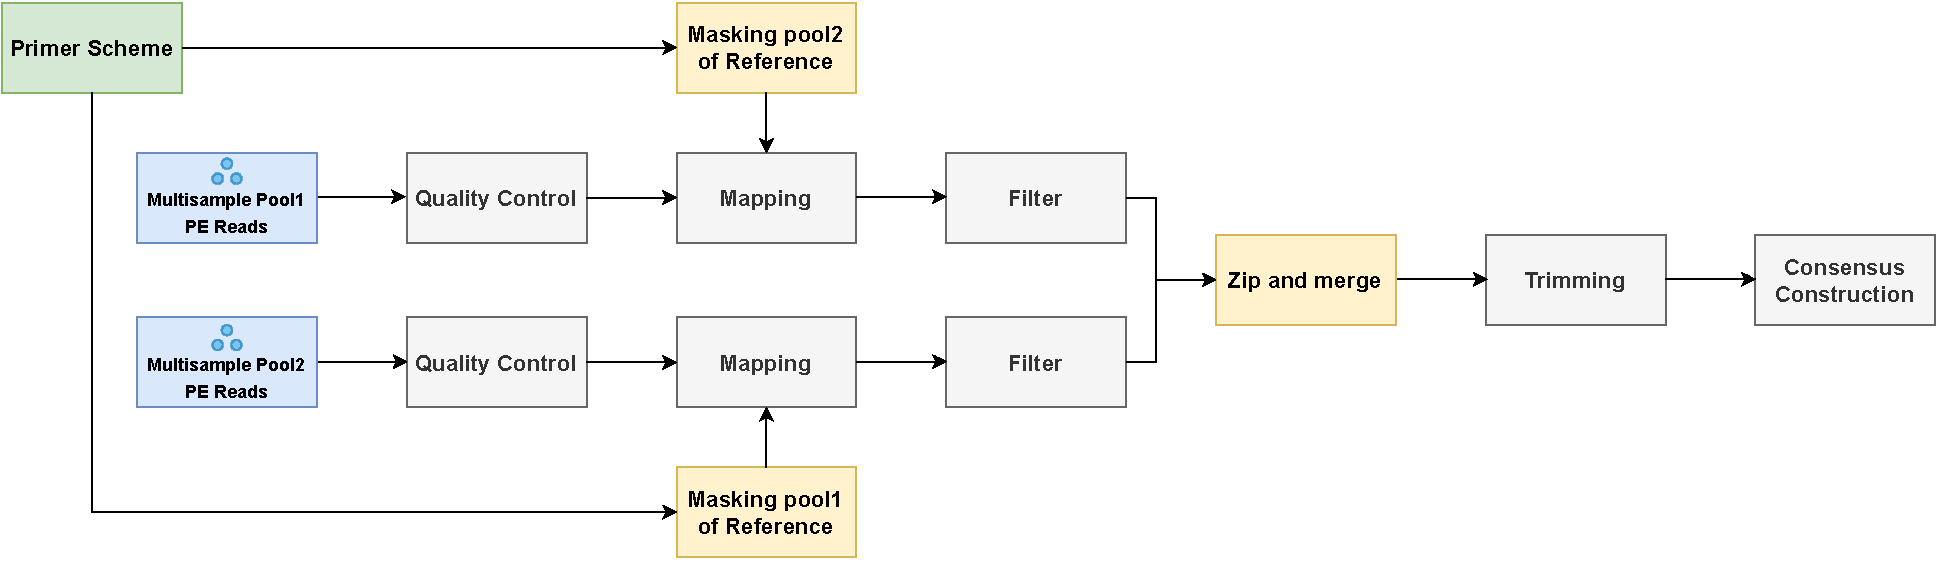
\includegraphics[width=0.97\textwidth]{media/3-pipelines-LSDV.pdf}
% 	\caption{Simplified Poxvirus PE reads iVar-based workflow.}
% 	\label{fig:3-pipelines-lsdv}
% \end{figure}

Efficiency: Assembly vs. Mapping; efficiency more details in discussion.

If the goal in a broad and rapid surveillance is a high number of sample throughput and analysis, assembly is too cost and time senstive. The presented pipeline could be used in a broad context for the use in many laboraties.
building index is expensive (BWT)

\subsection{AIV Illumina Reads Workflow}
We propose a fully automated pipeline for the analysis of Illumina-sequenced paired-end reads from influenza samples. The workflow is integrated in the Galaxy platform and available via \todo{link}. It is designed to take one input sample at a time and the outputs of the analysis steps can be used for further research based on the user's interest. The workflow is outlined in Figure~\ref{fig:3-aiv-wf}, where the nine main steps of the workflow are visualized. One upside of the workflow is the consideration of the different segments of the influenza virus genome. After uploading paired-end reads and a reference sequence database, which is available online too \todo{link}, the workflow is designed to build a hybrid reference from the given database for each of the segments of the genome. The reference sequence database consists of eight FASTA files, one per segment, containing numerous full-length sequences for a given segment. The provided database file consists of 56 sequences for each segment. If a user decides to upload their own references, it is important to follow the sequence identifier pattern: >\textit{segment\_name$\mid$influenza\_strain$\mid$subtype$\mid$accession\_number}. For example, one entry's identifier is >\textit{PB1$\mid$A/duck/Manitoba/1953$\mid$A/H10N7$\mid$KF435047.1} followed by the sequence. \\
After (1) preprocessing of the reads with \texttt{fastp} to dismiss reads shorter than 30 basepairs and trimming read ends, the database of reference sequences is used to (3) find the closest possible reference for each of the segments. The tool \texttt{VAPOR} outputs a table with a scoring that comes from the graph construction, and should not be confused with the identity of the sequence compared to the reference. As \texttt{VAPOR} is running once per segment but has independent inputs, this step is executed in parallel. \texttt{VAPOR} is a graph-based classifier that maps k-mers to a weighted De Bruijn graph~\cite{southgate2020influenza}. Its benchmarking shows that it runs significantly faster than BLAST and default configuration leads to reasonable matches, as long as the given sample is not very different from or novel to the provided sequences in the database. \\
Using the highest scoring sequences from the eight \texttt{VAPOR} runs, a hybrid reference sequence is built. To control the statistics of the graph and adapt the configuration, a table with the highest \texttt{VAPOR} scores of each run is generated. \\
The hybrid reference sequence is composed of the eight segments and is used for (3) mapping with \texttt{BWA-MEM} (Burrow-Wheeler Aligner for short-read alignment)~\cite{li2013aligning}. 

48 distinct steps

user can decide for size of phylogenetic trees (number of sequences to include from the next closer sequences -> measure by VAPOR scores, determines size of tree)

consensus sequence per segment is included in the phylogenetic trees to visualize the taxonomy (spatial/temporal spread)

upload list of FASTA files with a reference database for each influenza segment;

Table~\ref{tab:aiv-tools-steps}

\begin{figure}[H]
	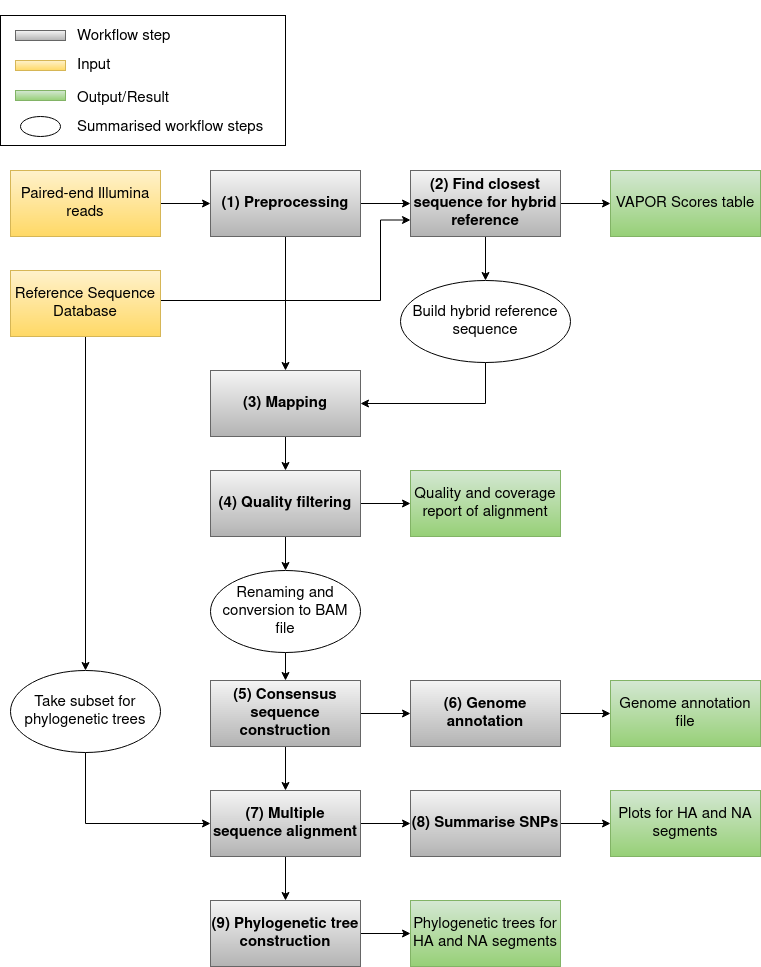
\includegraphics[width=0.95\textwidth]{media/aiv.png}
	\caption{Simplified AIV Illumina reads iVar-based workflow.}
	\label{fig:3-aiv-wf}
\end{figure}

steps:
(3) Mapping with BWA-MEM: preprocessed reads against hybrid reference, BAM output
(4) Filter by quality and for paired and properly mapped reads
(5) Consensus sequence construction (from BAM file with useful sequence names that include the segment name)
(-) create an overview of the VAPOR scoring in form of a table, with the identifier names
(6) Prokka from consensus sequences, for genome annotation (kingdom viruses)
(7) Snipit to visualize and summarize SNPs relative to the hybrid reference, needs a multiple sequence alignment of the segments with MAFFT
(8) IQ-Tree build phylogenetic tree from filtered reference database, size of the tree is determined by input, consensus sequences are renamed so they contain the segment name and the sample and outputs trees for HA and NA genes.

Overview of outputs in a table with datatypes
(1) Quality and coverage report of alignment
(2) VAPOR scores in a table
(3) Genome annotation file
(4) snipit SNP plots for HA and NA genes
(5) IQ-Trees for HA and NA genes

Kraken2 vs. VAPOR;
Efficiency: LoFreq vs. iVar consensus; both consensus identification methods using the same site-specific depth threshold

% \begin{figure}
% 	\centering
% 	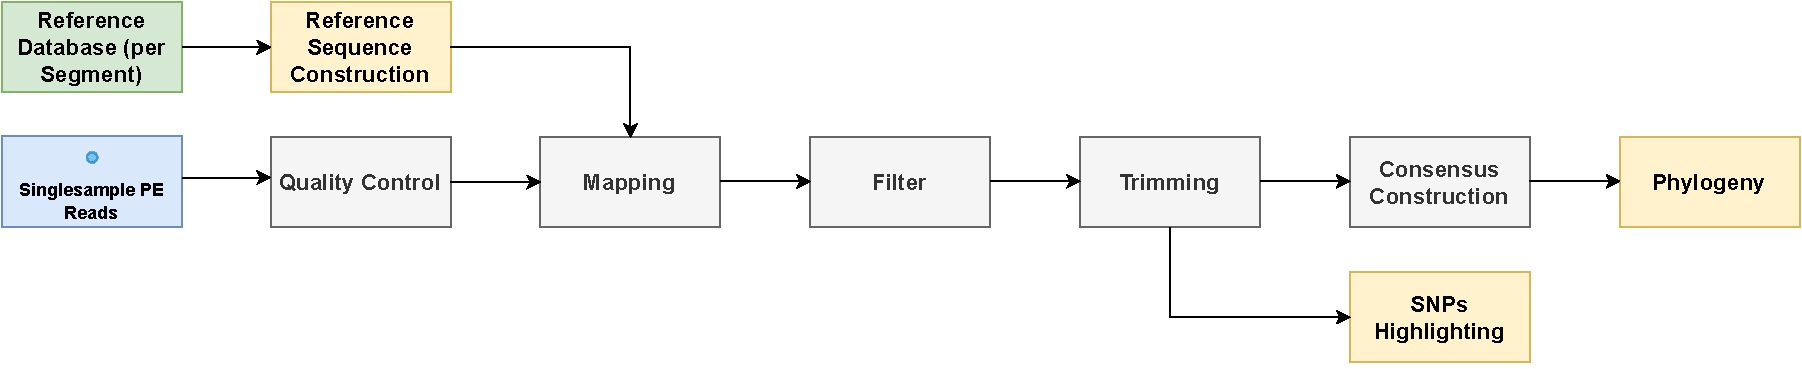
\includegraphics[width=0.97\textwidth]{media/3-pipelines-AIV.pdf}
% 	\caption{Simplified AIV ARTIC PE reads iVar-based workflow.}
% 	\label{fig:3-pipelines-aiv}
% \end{figure}

\subsection{FMDV Illumina Amplicon Workflow}
